\chapter{Pipeline Overview}\label{chapter:pipelineoverview}

\begin{figure}
  \centering
  
  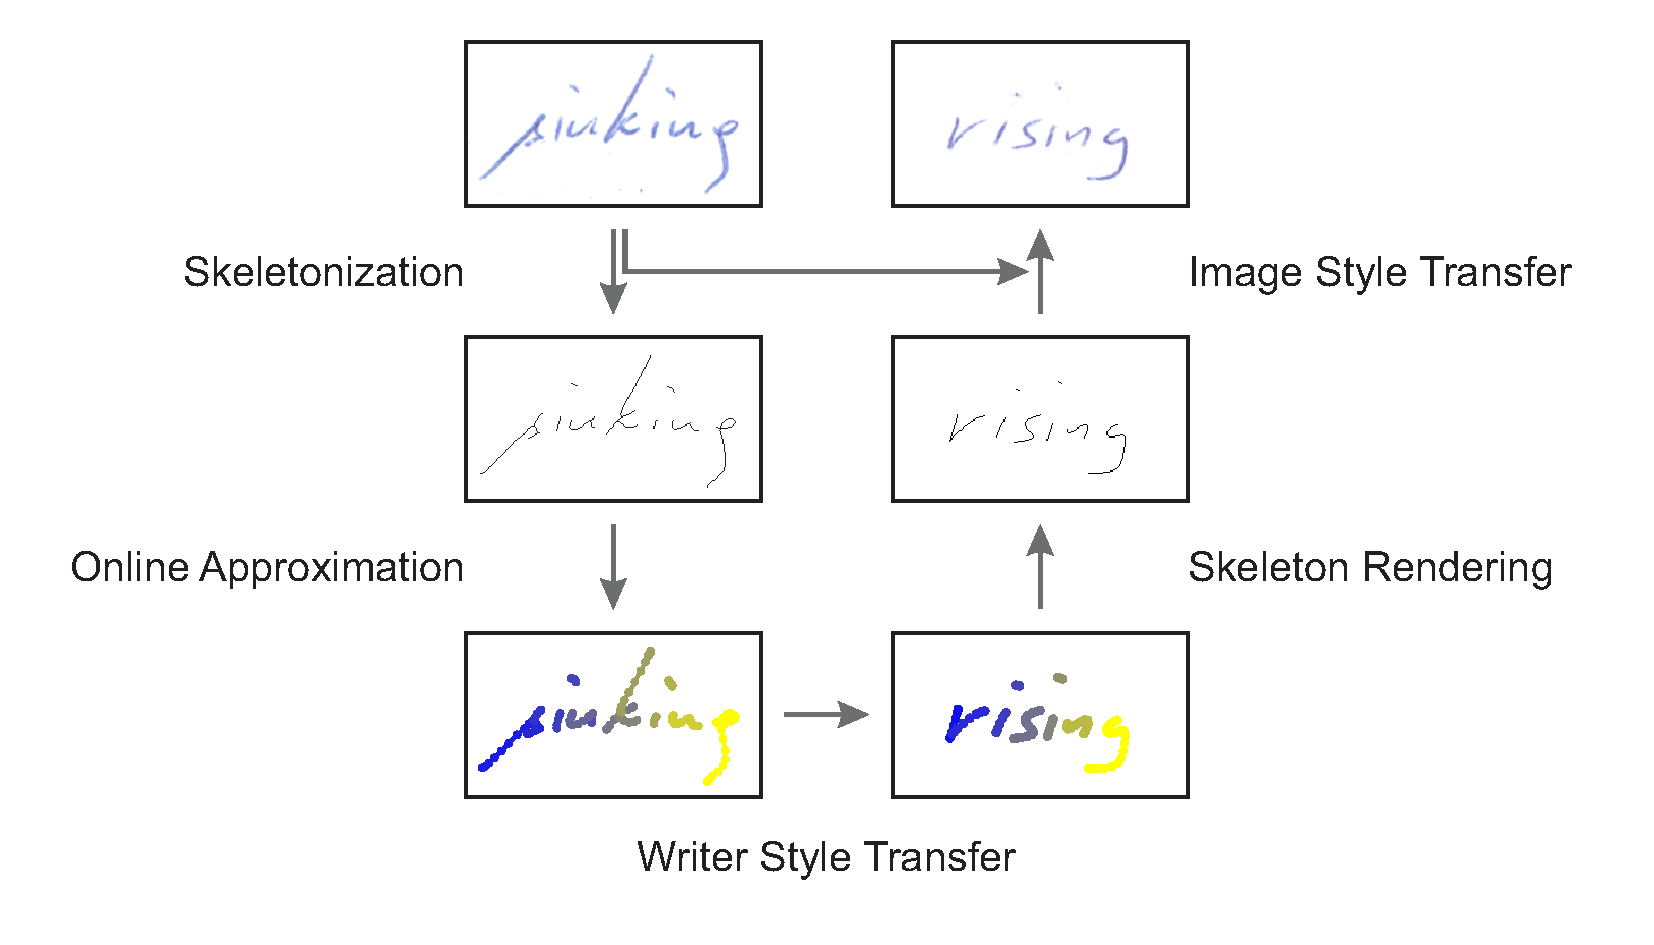
\includegraphics[width=0.95\textwidth]{../assets/pipeline.pdf}
  
  \caption[Overview of the style transfer pipeline]{Overview of the style transfer pipeline}
  \label{fig:styleTransferPipelineOverview}
\end{figure}


There are several reasons why the task of handwriting style transfer should be split into multiple steps instead of trying to create a neural network end-to-end solution. Neural networks are very good at fulfilling a single task, but as soon as this single task consists of multiple sub-steps, it becomes increasingly difficult for a neural network to figure out all of the steps at once, resulting in a network training without convergence. For handwriting style transfer, this complexity is quite obvious: The network would first have to learn the difference between the text and the meaningless background. It then has to grasp the concept of a stroke opposed to the color and type of the pen, and then further separate that into writer style and text content. Additionally, it has to remember the writer style, the color and type of the pen and the original background to produce a result with a style that matches the input image. To learn all of that at once without any guidance is almost impossible with the current type of networks. This is even more obvious when looking at the type of the content: While background, pen and writer style are static problems that could be solved with \glspl{cnn}, the text content has a sequential component and therefore requires some type of \gls{rnn}.

Another reason for splitting the problem into multiple stages is that most of those sub-problems are very well trainable on their own, allowing human prior knowledge to both guide the process as also to evaluate the single steps separately. Additionally, not all of those tasks require a neural network, some might even benefit from having an algorithmic solution. We therefore decided to break the problem down into a multi-staged pipeline.

\pagebreak
The proposed pipeline consists of the following five steps, as also seen in \cref{fig:styleTransferPipelineOverview}:
\begin{enumerate}[topsep=0pt,itemsep=-1ex,partopsep=1ex,parsep=1ex]
\item Skeletonization
\item Approximation of an online representation
\item Writer Style Transfer
\item Rendering to skeletons
\item Image Style Transfer
\end{enumerate}

\textbf{Skeletonization.}
This stage takes pictures of handwritten text and converts them to binary skeleton images. While this problem isn't something new, our use case requires a high degree of robustness. More specifically, the output skeleton images cannot contain salt and pepper noise and all lines must be connected continuously. This renders most traditional techniques insufficient and calls for new methods, which in our case was the utilization of a neural network. Provided with the correct training data, neural networks can become quite robust in understanding the actual content of an image opposed to simple thresholding or grouping.

\textbf{Approximation of an online representation.}
The core of this thesis is the utilization of existing online-to-online writer style transfer networks, which require an online representation of the handwriting. We therefore heuristically transform the offline data into an online format that the writer style transfer step can understand. As this step involves manually crafted heuristics, we did not train a neural network for it but instead hand-crafted an algorithmic solution.

\textbf{Writer Style Transfer.}
This stage takes the synthetic online representation, extracts the writer style and synthesizes new text in the given style. This step mostly utilizes the existing work of Graves.~\cite{graves}

\textbf{Rendering to skeletons.}
The next stage renders the online representation of the synthesized handwriting to offline skeletons. As this is simply a matter of drawing lines on a bitmap, it will not be discussed any further.

\textbf{Image Style Transfer.}
The purpose of this step is to take the generated skeletons and transform them into a realistic-looking image. At the moment of writing, lots of \gls{cnn} based solutions to similar problems produce excellent results, so we also utilized a \gls{cnn} based algorithm to produce those images. We tackled this step twice, first with colored text on a white background, and the second time including more realistic backgrounds. We achieve quite believable results without the backgrounds, but encounter problems as soon as we include them. Nonetheless, we analyze the problems and propose multiple possible solutions.



